\subsection{How to Implement Features?}
\begin{frame}{\myframetitle}
	\begin{mycolumns}
		\myexampletight{Given a feature model for graphs \ldots}{
			\centering\featureDiagramGraphs
			%\featureDiagramLegend
		}
		\myexample{\ldots\ we can derive a valid configuration}{
			\small
			\leftmiddleandright{
				$\{G\}$\\
				$\{G,C\}$\\
				$\{G,D\}$\\
				$\{G,C,D\}$\\
			}{
				$\{G,W\}$\\
				$\{G,C,W\}$\\
				$\{G,D,W\}$\\
				$\{G,C,D,W\}$\\
			}{
				$\{G,W,S\}$\\
				$\{G,C,W,S\}$\\
				$\{G,D,W,S\}$\\
				$\{G,C,D,W,S\}$\\
			}
		}
	\mynextcolumn
		\vspace{-10mm}
		\myexampletight{How to Generate Products Automatically?}{
			\centering\foreach \page in {2,12,4,14,6,16,8,18,10,20,42,44}{\includegraphics[width=.23\linewidth,page=\page]{graphs} }
		}
		\mynote{Goals}{
			\begin{itemize}
				\item descriptive specification of a product (i.e., a configuration, a selection of features)
				\item automated generation of a product with compile-time variability
			\end{itemize}
			Focus of the next three lectures \ldots
		}
	\end{mycolumns}
\end{frame}

\subsection{Problems of Ad-Hoc Approaches for Variability}

\subsubsection{Features with Runtime Variability?}
\begin{frame}[fragile]{\myframetitle}
	\footnotesize
	\begin{mycolumns}[animation=none]
\begin{codetight}{}
public class Config {
	~public static boolean COLORED = true;~
	@public static boolean WEIGHTED = false;@
}
\end{codetight}
\begin{codetight}{}
public class Graph {
	...
	Edge add(Node n, Node m) {
		Edge e = new Edge(n, m);
		nodes.add(n); nodes.add(m); edges.add(e);
		@if (Config.WEIGHTED) { e.weight = new Weight(); }@
		return e;
	}
	@Edge add(Node n, Node m, Weight w) {
		if (!Config.WEIGHTED) { throw new RuntimeException(); }
		Edge e = new Edge(n, m);
		nodes.add(n); nodes.add(m); edges.add(e);
		e.weight = w;
		return e;
	}@
	...
}
\end{codetight}
	\mynextcolumn
\begin{codetight}{}
public class Node {
	~Color color;~
	...
	Node(){
		~if (Config.COLORED) { color = new Color(); }~
	}
	void print() {
		~if (Config.COLORED) { Color.setDisplayColor(color); }~
		System.out.print(id);
	}
}
\end{codetight}
\begin{codetight}{}
public class Edge {
	@Weight weight;@
	...
	Edge(Node _a, Node _b) {
		a = _a; b = _b;
		@if (Config.WEIGHTED) { weight = new Weight(); }@
	}
	void print() {
		a.print(); b.print();
		@if (Config.WEIGHTED) { weight.print(); }@
	}
}
\end{codetight}
	\end{mycolumns}
\end{frame}

\begin{frame}{\myframetitle}
	\begin{mycolumns}[widths={40},T]
		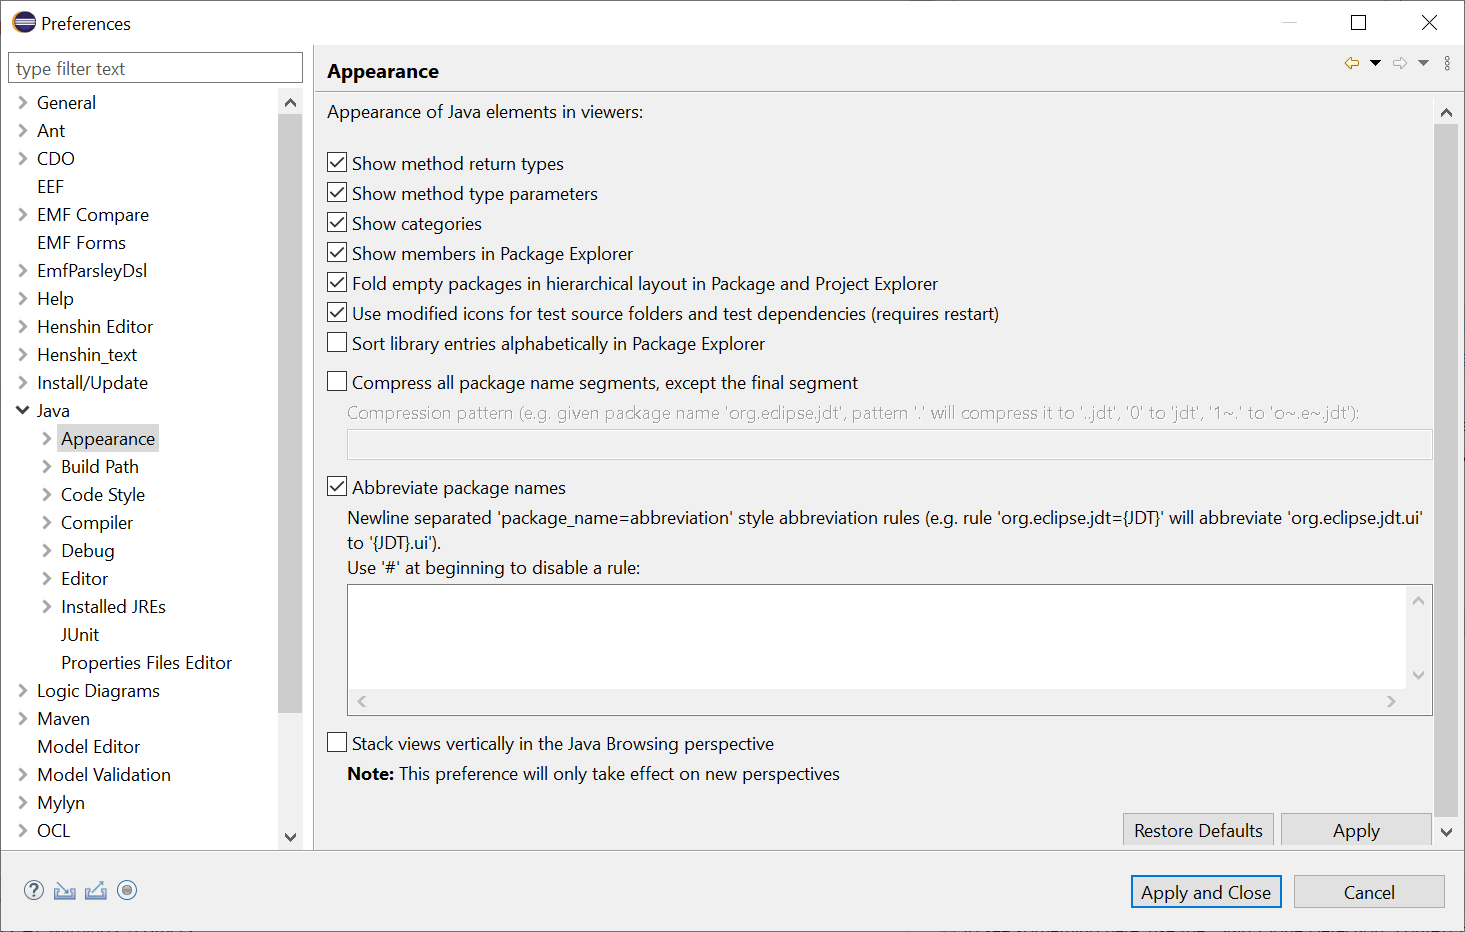
\includegraphics[width=\linewidth]{preferences-eclipse}

		\begin{definition}{How to? -- Preference Dialog}
			\begin{itemize}
				\item implement runtime variability
				\item compile the program
				\item manually adjust preferences based on configuration
				\item run the program
			\end{itemize}
		\end{definition}
	\mynextcolumn
		\leftandright{
			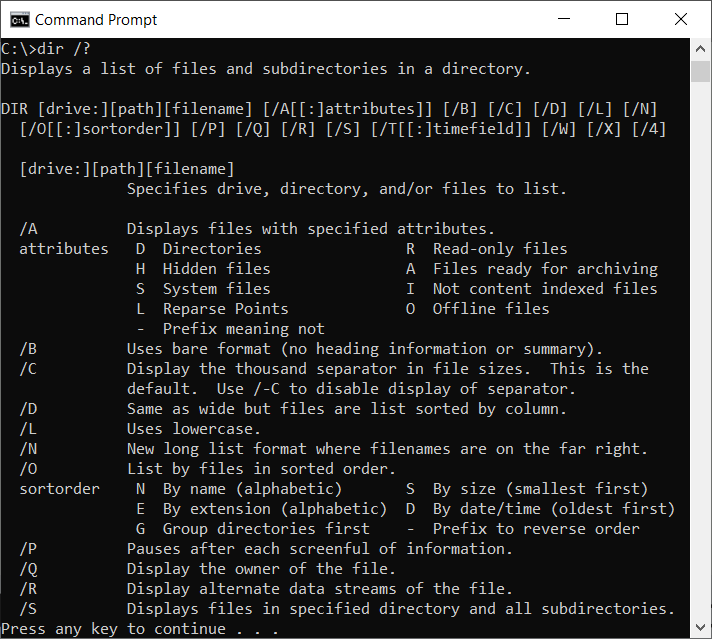
\includegraphics[width=\linewidth]{runtime-parameters-win10-cmd-dir}
		}{
			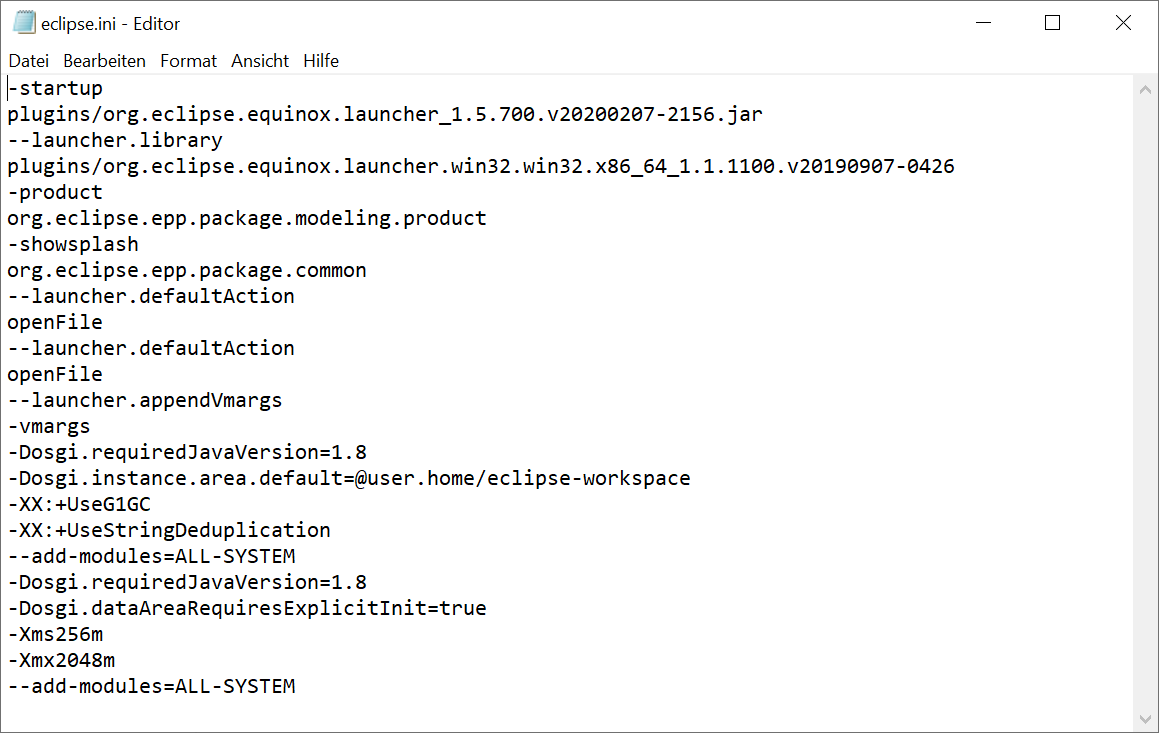
\includegraphics[width=\linewidth]{configfile-eclipse-ini}
		}

		\begin{definition}{How to? -- Command-Line Options / Configuration Files}
			\begin{itemize}
				\item implement runtime variability
				\item compile the program
				\item automatically generate command-line options / configuration files based on configuration
				\item run the program
			\end{itemize}
		\end{definition}
	\end{mycolumns}
\end{frame}

\begin{frame}[fragile]{\myframetitle}
	\begin{mycolumns}[widths={48}]
\begin{codetight}[basicstyle=\small]{}
public class Config {
	~public final static boolean COLORED = true;~
	@public final static boolean WEIGHTED = false;@
}
\end{codetight}
		\begin{definition}{How to? -- Immutable Global Variables}
			\begin{itemize}
				\item implement runtime variability
				\item automatically generate class with global variables based on configuration
				\item compile and run the program
			\end{itemize}
		\end{definition}
	\mynextcolumn
		\begin{note}{What is missing?}
			\begin{itemize}
				\item automated generation:\\\hfill for preference dialogs
				\item no compile-time variability / same large binary:\\\hfill for all except immutable global variables
				\item very limited compile-time variability:\\\hfill for immutable global variables
			\end{itemize}
		\end{note}
	\end{mycolumns}
\end{frame}

\subsubsection{Features with Clone-and-Own?}
\begin{frame}{\myframetitle}
	\begin{mycolumns}[widths={30}]
		\centering~

		
\includegraphics[scale=0.2]{alice}
		\includegraphics[scale=0.26,page=2]{graphs}

		
\includegraphics[scale=0.2]{bob}
		\includegraphics[scale=0.26,page=12]{graphs}

		
\includegraphics[scale=0.2]{eve}
		\includegraphics[scale=0.26,page=16]{graphs}
	\mynextcolumn
		\begin{definition}{How to?}
			\begin{itemize}
				\item implement separate project for each product\\(i.e., branch with version control)
				\item download project / checkout branch based on configuration
				\item run build script, if existent
				\item compile and run the program
			\end{itemize}
		\end{definition}
		\begin{note}{What is missing?}
			\begin{itemize}
				\item compile-time variability only for implemented products
				\item no automated generation:\\\hfill for clone-and-own (with version control systems)
				\item automated generation based on build script and extra files:\\\hfill for clone-and-own with build systems
				\item no free feature selection (i.e., configuration)
			\end{itemize}
		\end{note}
	\end{mycolumns}
\end{frame}

\subsection{Recap: Clone-and-Own with Build Systems}
\begin{frame}{\myframetitle\  \mytitlesource{\href{https://dl.acm.org/doi/10.1145/3461002.3473950}{Kuiter~et~al.~2021}}}
	\begin{mycolumns}[columns=2,widths={65},animation=none]
		\centering
			\leftandright{
				\myexample{\small Case Study: Anesthesia Device}{
					\begin{itemize}
						\item C application
						\item targets embedded devices (ESP32)
						\item configurations are hard-coded as build scripts
					\end{itemize}
				}
			}{
				\uncover<4->{\myexampletight{\small{\color{red}Production Device}: OLED, Clock}{\pic[width=\linewidth]{pignap-cfg-production-oled}}}
			}

			\leftandright{
				\uncover<2->{\myexampletight{\small{\color{green}Prototype}: OLED Display}{\pic[width=\linewidth]{pignap-cfg-prototype-oled}}}
			}{
				\uncover<3->{\myexampletight{\small{\color{blue}Prototype}: LCD, Real-Time Clock}{\pic[width=\linewidth]{pignap-cfg-prototype-lcd-rtc}}}
			}
		\mynextcolumn
			\centering
			\only<1>{\pic[width=.65\linewidth,page=1]{pignap-variants}}%
			\only<2>{\pic[width=.65\linewidth,page=2]{pignap-variants}}%
			\only<3>{\pic[width=.65\linewidth,page=3]{pignap-variants}}%
			\only<4>{\pic[width=.65\linewidth,page=4]{pignap-variants}}
	\end{mycolumns}
\end{frame}

\subsection{Introducing Features to Build Systems}
\begin{frame}{\myframetitle\  \mytitlesource{\href{https://dl.acm.org/doi/10.1145/3461002.3473950}{Kuiter~et~al.~2021}}}
	\begin{mycolumns}[widths={60}]
		\mydefinition{How to Implement Features with Build Systems?}{
			\begin{itemize}
				\item step 1: model variability in a feature model
				\item step 2: in build scripts, in- and exclude files based on feature selection
				\item step 3: pass a feature selection at build time
			\end{itemize}
			$\Rightarrow$ one build script per group of related features
		}
		\myexampletight{}{
			\centering
			\featureDiagram{Anesthesia Device,abstract
			[Monitoring,abstract,mandatory
				[Display,abstract,or[LCD,concrete,alternative][OLED,concrete]]
				[Wi-Fi,abstract
					[HTTP Server,concrete,mandatory]]]
			[History,optional,concrete]
			[Libraries,abstract,mandatory
				[Storage,abstract,optional[NVS,concrete,alternative][FRAM,concrete]]
				[RTC,concrete,optional[Battery,concrete,mandatory]]]}

			$History \pimplies Storage \pand RTC$
		}
	\mynextcolumn
		\myexampletight{}{
			\centering
			\pic[width=.65\linewidth]{pignap-features}
		}
\end{mycolumns}
\end{frame}

\subsection{KBuild -- The Linux Kernel Build System}
\begin{frame}[fragile]{\myframetitle}
	\begin{mycolumns}
		\begin{kconfigtight}[basicstyle=\footnotesize]{Feature Model with KConfig\mysource{\href{https://github.com/torvalds/linux/blob/0326074/arch/x86/Kconfig}{linux/arch/x86/Kconfig}}}
config X86_32 ...
config X86_64 ...

config IA32_EMULATION
	bool "IA32 Emulation"
	depends on X86_64
	help Include code to run legacy 32-bit programs under a 64-bit kernel. You should likely enable this, unless you're 100% sure that you don't have any 32-bit programs left.
\end{kconfigtight}
		\mydefinition{KBuild\mysource{\href{https://www.kernel.org/doc/html/latest/kbuild/makefiles.html}{kernel.org}}}{
			\begin{itemize}
				\item a style for writing Makefiles in Linux
				\item defines goals with Make variables
				\begin{itemize}
					\item \texttt{obj-y}: static linkage (= include feature)
					\item \texttt{obj-m}: dynamic linkage (= as module)
					\item \texttt{obj-}: no linkage (= exclude feature)
				\end{itemize}
				\item full power of Make $\Rightarrow$ hard to comprehend
			\end{itemize}
		}
	\mynextcolumn
		\begin{kbuildtight}[basicstyle=\small]{Feature Mapping with KBuild \mysource{\href{https://github.com/torvalds/linux/blob/0326074/arch/x86/Kbuild}{linux/arch/x86/Kbuild}}}
# link these subdirectories statically:
obj-y += entry/ # entry routines
obj-y += realmode/ # 16-bit support
obj-y += kernel/ # x86 kernel
obj-y += mm/ # memory management

# link these depending on a configuration option:
obj-~$(CONFIG_IA32_EMULATION)~ += ia32/
obj-~$(CONFIG_XEN)~ += xen/ # paravirtualization

# the KConfig feature model can even be overridden:
obj-~$(subst m,y,$(CONFIG_HYPERV))~ += hyperv/
		\end{kbuildtight}

		\begin{kbuildtight}[basicstyle=\small]{Recurse into Subsystems\mysource{\href{https://github.com/torvalds/linux/blob/0326074/arch/x86/ia32/Makefile}{linux/arch/x86/ia32/Makefile}}}
# ia32 kernel emulation subsystem
obj-~$(CONFIG_IA32_EMULATION)~ := ia32_signal.o
audit-class-~$(CONFIG_AUDIT)~ := audit.o

# IA32_EMULATION and AUDIT required for audit.o:
obj-~$(CONFIG_IA32_EMULATION)~ += ~$(audit-class-y)~
		\end{kbuildtight}
	\end{mycolumns}
\end{frame}

\begin{frame}[fragile]{\myframetitle}
	\begin{mycolumns}
		\mynote{Recap: Interactive Linux Kernel Configurator}{\pic[width=\linewidth]{linux-menuconfig-emulation}}

		\begin{kconfigtight}[basicstyle=\footnotesize]{Feature Model and Example Configuration}
			config AUDIT ... # configured as NO
			config IA32_EMULATION ... # configured as YES
			config HYPERV ... # configured as MODULE
			config XEN ... # configured as NO
\end{kconfigtight}
	\mynextcolumn
		\begin{kbuildtight}[basicstyle=\small]{Feature Mapping}
obj-y += entry/ realmode/ kernel/ mm/
obj-~$(CONFIG_IA32_EMULATION)~ += ia32/
obj-~$(CONFIG_XEN)~ += xen/
obj-~$(subst m,y,$(CONFIG_HYPERV))~ += hyperv/
obj-~$(CONFIG_IA32_EMULATION)~ := ia32_signal.o
audit-class-~$(CONFIG_AUDIT)~ := audit.o
obj-~$(CONFIG_IA32_EMULATION)~ += ~$(audit-class-y)~
		\end{kbuildtight}

		\begin{kbuildtight}[basicstyle=\small]{Feature Mapping for Example Configuration}
obj-y += entry/ realmode/ kernel/ mm/
obj-?y? += ia32/
obj- += xen/
obj-?y? += hyperv/
obj-?y? := ia32_signal.o
audit-class- := audit.o
obj-?y? +=
		\end{kbuildtight}

		\mynote{}{\small i.e., \texttt{entry, realmode, kernel, mm, ia32, hyperv, ia32\_signal.o} are compiled}
	\end{mycolumns}
\end{frame}


\subsection{Discussion of Features with Build Systems}
\begin{frame}{\myframetitle}
	\begin{mycolumns}
		\mynote{Advantages}{
			\begin{itemize}
				\item compile-time variability\\
					$\Rightarrow$ \emph{fast, small binaries} with smaller attack surface and without disclosing secrets
				\item automated generation of arbitrary products\\
					$\Rightarrow$ \emph{free feature selection}
				\item allows in- and exclusion of individual files or even entire subsystems\\
					$\Rightarrow$ high-level, \emph{modular variability}
			\end{itemize}
		}
	\mynextcolumn
		\mynote{Challenges}{
			\begin{itemize}
				\item not easily reconfigurable at run- or load-time
				\item build scripts may become complex, there is no limit to what can be done (e.g., you can run arbitrary shell commands on files)\\
					$\Rightarrow$ \emph{hard to understand and analyze}
				\item no simple in- and exclusion of individual lines or chunks of code\\
				$\Rightarrow$ high-level use \emph{only}!
			\end{itemize}
		}
	\end{mycolumns}
\end{frame}
